\section{Introduction}
\label{sec:introduction}

A central path supplies both a route to an optimum and a scale for taking
locally controlled steps. The route need not be shortest in the metric
that controls those steps. To quantify the difference, one must specify
what a competing route must accomplish: reach the same central point,
reach any point with the same objective accuracy, or return a feasible
primal--dual pair with a small gap. These requirements lead to different
answers even for one sparse linear program on an ordinary cube.

We study these answers in the real Hessian metric of a specified
self-concordant barrier. A permitted move from $x$ to $y$ has bounded
starting local norm, $\norm{y-x}_{F,x}\leq R$, for fixed $0<R<1$.
The minimum number of such moves is comparable to metric distance,
up to integer rounding, with explicit constants depending only on $R$.
This permits a direct
comparison of centrality with the amount of movement actually needed
for accuracy. The principal example has three scales:
\[
 \underbrace{r\sqrt{\log r}}_{\text{arbitrary primal movement}},
 \qquad
 \underbrace{r\log r}_{\text{central primal movement}},
 \qquad
 \underbrace{r^{3/2}}_{\text{feasible primal--dual movement}}.
\]
The objective and tolerance are rational with polynomial ordinary
encoding length. The first separation persists for iterates in a fixed
central neighborhood, even when their reference central parameters
backtrack. The second separation applies to every feasible terminal dual
certificate in the specified product metric.

These are geometric comparisons, not operation counts. For example, a
linear objective on a box can be optimized by reading its signs, and a
spectral decomposition solves the corresponding support problem on a
matrix ball. The examples isolate costs imposed by a movement rule.
They do not imply a lower bound for algorithms permitted to bypass that
rule, or an arithmetic or oracle advantage for a general optimization
method.

\subsection{Results and the mechanism behind them}

The basic barrier is $U(x)=\sum_i b(x_i)$ on $(-1,1)^r$, where
$b(t)=-\log(1-t^2)$. Its scalar metric coordinate is
$\rho(t)=\int_0^t\sqrt{b''(u)}\dd u$.
In the coordinates $y_i=\rho(x_i)$, distances are Euclidean and shortest
paths are straight. A central path for a positive linear objective has
coordinates $y_i(s)=H(s-a_i)$, where $s$ is logarithmic central parameter,
$a_i$ is determined by the objective weight, and the common velocity
$H'$ increases from zero to one. Widely separated $a_i$ activate
successive groups of coordinates. The central curve bends through these
successive directions, whereas the shortest route moves them together.
\Cref{fig:flattened} illustrates this mechanism.

\begin{figure}[tbp]
 \centering
 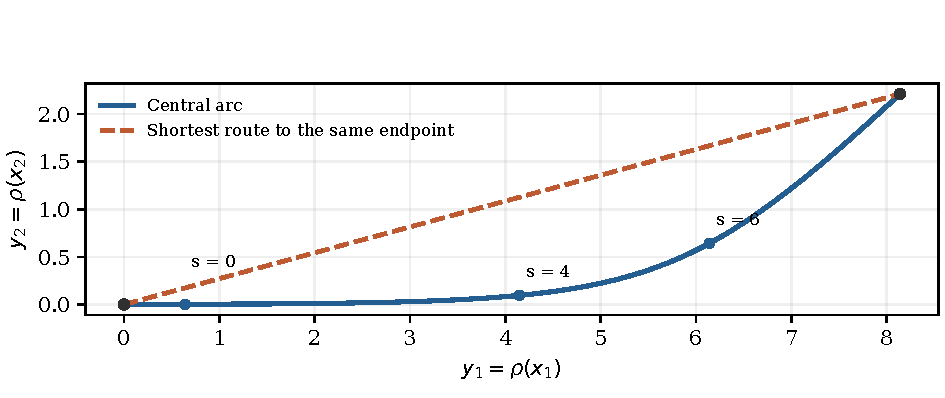
\includegraphics[width=.82\textwidth]{figures/flattened-path.pdf}
 \caption{A two-coordinate example in the exact metric coordinates
 $y_i=\rho(x_i)$. The barrier is $b(x_1)+b(x_2)$, objective weights are
 $(1,e^{-6})$, and the terminal logarithmic parameter is $s=8$.
 The central arc starts at the analytic-center limit $s=-\infty$.
 The straight segment is a globally shortest route to the same endpoint.
 The plot illustrates endpoint geometry; it does not display the closest
 point in an objective target set.}
 \label{fig:flattened}
\end{figure}

Our main results develop this mechanism in four directions.
\begin{enumerate}[leftmargin=*,label=\arabic*.]
\item \emph{Exact spectral geometry and the sharp rank factor.}
For rectangular real or complex spectral-norm balls and spectral
intervals in every Euclidean Jordan algebra, equipped with their standard
log-determinant barriers, distance from the analytic center is exactly
the Euclidean norm of the transformed singular values
or eigenvalues. Leaving the objective's spectral frame cannot shorten
this route. Distance to the entire accurate target set reduces to a
strictly convex scalar allocation with one multiplier
(\cref{thm:exact-distance,thm:water-filling}).
For equal barrier scales and $r$ active objective channels, every central
subarc satisfies
\begin{equation}
 L_{\CP}\leq\Gamma_r d_F(\text{its endpoints}),\qquad
 \Gamma_r=\left[\sum_{i=1}^r(\sqrt i-\sqrt{i-1})^2\right]^{1/2},
 \qquad \Gamma_r^2=\tfrac14\log r+O(1).
 \label{eq:intro-Gamma}
\end{equation}
The supremum of this ratio is exactly $\Gamma_r$.
For the same objective accuracy,
$L_{\CP}(\eps)\leq c_\star\Gamma_r L_\opt(\eps)$,
where $1.37486<c_\star<1.38$ is the sharp constant in a specified scalar
KKT comparison, certified by rational arithmetic. Sharpness of the
product $c_\star\Gamma_r$ is not asserted
(\cref{thm:sharp-prefix,thm:scalar-dilation}).
Unequal factor scales give an exact weighted prefix constant; its value
depends on activation order and can have order $\sqrt r$ when the scale
range grows exponentially (\cref{prop:scale-order}).

\item \emph{A separation for actual finite sequences.}
An explicit dyadic objective and tolerance on the cube give
$L_\opt=\Theta(r\sqrt{\log r})$ and
$L_\CP=\Theta(r\log r)$, with ordinary input length
$\Theta(r^2)$ (\cref{thm:dyadic}). A clipped progress function proves
that every forward-$R$ sequence in a fixed metric tube around the
central path needs $\Omega(r\log r)$ moves to attain actual accuracy,
with a matching $O(r\log r)$ construction.
The labels may be arbitrary and nonmonotone; no sampling assumption is
imposed on the competing sequence. More generally, a diverging overhead
survives tube radii $\delta_r=o((\log r)^{1/3})$
(\cref{thm:tube}). Fixed Newton-decrement neighborhoods of radius
$0\leq\beta<1/2$ satisfy this contract. The distinction between central arclength and finite sequences
is necessary: an arclength lower bound alone does not exclude chords
that skip a long part of a curve.

\item \emph{Persistence beyond the standard separable barrier.}
Every fixed scalar barrier satisfying the positive-branch normalization
$(f')^2\leq f''$ has the same sharp endpoint factor $\Gamma_r$,
a uniform same-accuracy comparison with constant $C_{\SC}<2$, and the
same dyadic separation. This includes the universal and entropic cube
barriers (\cref{thm:normalized-scalar,prop:canonical-cube}).
The scalar normalization has content: the unrestricted class admits
ratios approaching $\sqrt r$, with a growing scalar parameter.
Convex couplings with bounded first and second derivatives on one full
facet collar retain a worst ratio at least $\Gamma_r$
(\cref{thm:facet-coupling}). We give dense and fully signed-permutation
invariant coupled examples with exact, optimal cube parameter $r$.
For the explicit radial family
\[
 F_{\lambda,c}(x)=U(x)-\lambda\log(c-\norm x^2),
 \qquad \lambda\geq1,\quad c-r\geq4\lambda,
\]
we also prove a matching $O(\Gamma_r)$ upper comparison and uniform
persistence of the finite-sequence separation, even when $\lambda,c$
vary with dimension (\cref{thm:radial-upper,cor:radial-discrete}).
Thus optimal parameter and substantial symmetry do not ensure a bounded
centrality ratio. The matching upper theorem concerns this explicit
family; the facet-collar theorem for general couplings is a lower bound.

\item \emph{The additional cost of a dual completion.}
Classical primal--dual geometry fixes total central speed at $\sqrt\nu$
in logarithmic parameter. We calculate how objective activity divides
this speed between primal and dual components. An optimal product-ball
cone barrier permits much less primal movement than its parameter alone
would suggest, even with positive weights and a unique projected
optimizer. Most directly, the same dyadic sparse LP has optimal primal
movement $\Theta(r\sqrt{\log r})$, central primal movement
$\Theta(r\log r)$, and movement to any feasible full small-gap point
$\Theta(r^{3/2})$ (\cref{thm:completion}). The metric and endpoint
contracts are stated separately in that theorem.
\end{enumerate}

The supporting results identify when these comparisons survive additional
structure. Effective objective rank gives explicit velocity and error
laws, including geometric and polynomial spectral decay; a determinant
rank certificate can miss an unbounded target distance
(\cref{sec:distribution}). For changes of formulation, an exposed
Jordan minor gives a weighted support-rank lower bound that allows all
auxiliary fibers to move. A dimension cap on operational cone factors
gives a full primal--dual lower bound for arbitrary logarithmically
homogeneous barriers. Grouped balls, norm trees and arbitrary PSD column
packing provide complete fixed-metric examples, including exact restricted
parameters and heterogeneous objective scales
(\cref{sec:formulation,app:formulations}). These consequences distinguish
which information comes from the objective, the barrier, and the lift.

\subsection{Relationship to prior work}
\label{subsec:geometric-prior}

Nesterov and Todd~\cite{NesterovTodd2002} established the basic
Riemannian geometry of self-concordant barriers, its connection to bounded
local steps, and the product rule for distances. Their Section~6.2
flattens a separable hypercube metric by integrating its scalar local
norm. Their primal--dual theorem bounds central length by $\sqrt2$ times
endpoint distance in the metric of a logarithmically homogeneous cone
barrier plus its conjugate. Their Theorem~5.1(c) and Corollary~5.1 already
extend the comparison to the entire feasible small-gap set, with possible
affine infeasibility at intermediate points. We restate this classical
result in \cref{thm:pd-gap-set} to make the contrast with primal shortcuts
precise; the gap-set extension is not an original contribution.

Nesterov and Nemirovski~\cite{NesterovNemirovski2008} studied primal
central paths versus geodesics. If $D$ is the distance between two
central points, their Theorem~4.1 gives
\begin{equation}
 L\leq\log2+\nu^{1/4}\sqrt{D(D+\log12)}.
 \label{eq:NN-comparison}
\end{equation}
Their Example~1.1 distinguishes a central endpoint from an objective
target set, and their Theorem~5.3 gives a target-set comparison under
an explicit separation assumption. The present work addresses that
established comparison problem on specified spectral domains: it
computes the accurate-target benchmark and replaces the general
parameter dependence by an exact active-rank constant for these metrics.

Worst-case central-path behavior and lower bounds for path-following
methods have a substantial separate history. Deza, Nematollahi and
Terlaky~\cite{DezaNematollahiTerlaky2008} study iteration lower bounds
through Klee--Minty constructions. Allamigeon, Benchimol, Gaubert and
Joswig~\cite{AllamigeonEtAl2018} construct long-winding logarithmic
central paths and prove exponential neighborhood iteration lower bounds.
Allamigeon, Gaubert and
Vandame~\cite{AllamigeonGaubertVandame2022} give exponential lower bounds
for self-concordant-barrier path-following methods in their prescribed
neighborhood model. Allamigeon, Dadush, Loho, Natura and
V\'egh~\cite{AllamigeonEtAl2025} compare an interior-point method with
\emph{straight-line complexity}, which counts affine segments in a wide
central neighborhood, and obtain comparisons across self-concordant
barriers. Dadush, Ma, Natura and V\'egh~\cite{DadushMaNaturaVegh2026}
improve wide-neighborhood guarantees expressed in terms of straight-line
complexity and establish approximate instance optimality of trust-region
path following in the narrow $\ell_2$ neighborhood. Their affine-segment
and algorithmic iteration resources differ from the fixed-radius
local-Hessian moves counted here. Our dyadic example gives a separation between
central-neighborhood movement and unrestricted target distance in the
same metric on the same simple domain; it is not a first demonstration
of central-path inefficiency or a barrier-independent exponential
iteration lower bound.

Several ingredients have direct classical antecedents. The prefix norm
inequality is a finite weighted Lorentz-norm inequality
\cite{Lorentz1951}; the new comparison requires its sharp realization by
translated central velocities. The matrix and Jordan Hessian calculations
use spectral differentiation~\cite{LewisSendov2001,Baes2007}.
Metric projections and conjugate Hessian isometries appear explicitly
in Ohara, Ishi and Tsuchiya~\cite{OharaIshiTsuchiya2024}.
The universal and entropic constructions and their exact dimension
parameters are due to earlier work
\cite{NesterovNemirovskii1994,LeeYue2021,BubeckEldan2019,Chewi2023};
we derive their centrality consequences. Parameter-preserving diagonal
quadratic regularization on boxes is also prior work
\cite{CastroCuesta2011}. The coupled examples here supplement that
construction literature with exact-parameter path comparisons.

Geodesic updates in symmetric-cone algorithms
\cite{Permenter2023} and interior-point methods on Riemannian base
manifolds~\cite{HiraiNieuwboerWalter2026} concern complementary algorithmic
settings. The real Hessian metric on a bounded spectral ball used here
is distinct from the affine-invariant metric on a symmetric cone and
from complex Bergman metrics. The formulas are proved for the stated
metric, including complex matrix spaces viewed as real vector spaces.

To the best of our knowledge, the exact active-rank supremum
\eqref{eq:intro-Gamma} for these central paths, its combination with the
explicit accurate-target allocation, the dyadic finite-sequence
separation with arbitrary labels, the uniform comparison for the stated
radial coupled family, and the same-instance three-scale completion
comparison have not appeared in the cited literature. These are the
specific original claims supported by our proofs and literature review.
The general geometric framework, canonical barriers, and classical
primal--dual gap-set comparison are antecedents of these results.

\subsection{Organization}
\Cref{sec:foundations} fixes the metric and local-step conventions.
\Cref{sec:exact-distance,sec:sharp-centrality} establish the exact
benchmark and sharp comparison; \cref{sec:distribution,sec:discrete}
develop objective profiles and finite sequences.
\Cref{sec:barrier-dependence,sec:coupled-barriers} treat scalar and
coupled changes of barrier. \Cref{sec:primal-dual,sec:formulation}
separate dual completion from formulation effects.
The appendices give the rational scalar certificate, the normalized
profile envelope and nonmonotone construction, and the complete proofs
for the concrete formulations. The figures are reproducible numerical
illustrations of analytically proved results.
